Here we introduce a few Poncelet triangle families interscribed in non-concentric, axis-parallel (NCAP) ellipse pairs. In some of the families below, at least one of the ellipses is a circle, so perhaps ``co-axial'' could also be employed.

\subsection{Poristic Family (Bicentric Triangles)}

\begin{figure}
    \centering
    %\includegraphics[width=\textwidth]{pics/0010x_obtuse_poristics.eps}
    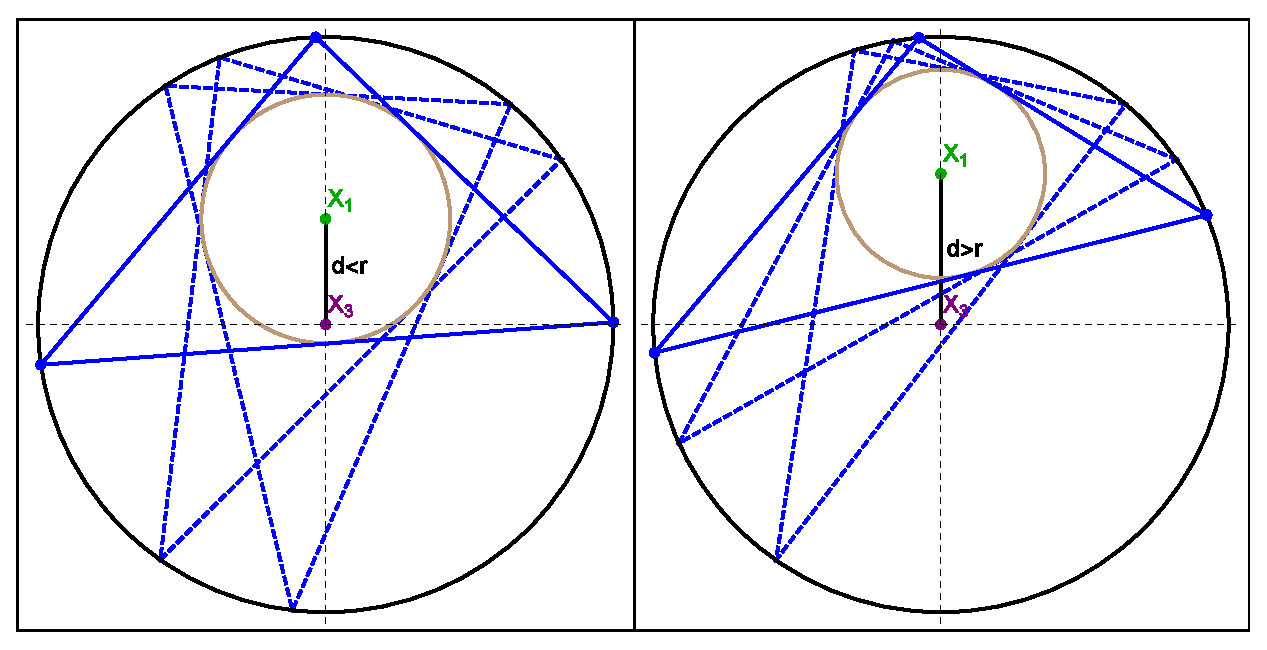
\includegraphics[width=\textwidth]{
    pics_03_180_obtuse_poristics.eps}
    \caption{Poristic Triangle family (blue): fixed incircle (green) and circumcircle (purple). \textbf{Left}: a few poristic triangles (blue and dashed blue) in a pair of circles such that $d<r$, i.e.,  all poristic triangles are acute. \textbf{Right}: the same but with $d>r$; since $X_3$ can be either interior or exterior to the family, both acute and obtuse triangles will be present. \href{https://bit.ly/3bg19iD}{Live}}
    \label{fig:03-poristic obtuse}
\end{figure}

Poristic triangles, shown in \cref{fig:03-poristic obtuse}, are the simplest case of Poncelet's porism: a 1d family of triangles with fixed incircle and circumcircle. They are they $N=3$ case of the bicentric family covered in \cref{chap:06-bicentric}.

First described by \cite{chapple1746-poristics}, the family was later studied by both Euler and Poncelet. The so-called Euler's triangle formula\footnote{Chapple had stated it in 1746, Euler in 1765, and Poncelet's porism was published in 1822; see \cite{centina15}.}, constrains the distance $d$ between incenter $X_1$ and circumcenter $X_3$ as follows:

\begin{equation}
d^2=R(R-2 r)
\label{eq:03-euler-poristic}
\end{equation}
where $r,R$ are the radii of outer and inner circle.

Referring to \cref{fig:03-poristic obtuse}:

\begin{proposition}
The Poristic family will contain obtuse triangles iff $d>r$.
\end{proposition}

\begin{proof}
This stems from the fact that when $d<r$, $X_3$ is always interior to the incircle, i.e., the caustic of the Poncelet family. 
\end{proof}

In consonance with both billiard 3-periodics and the incircle family:

\begin{proposition}
The poristic family conserves the sum of its internal angle cosines.
\end{proposition}

\begin{proof}
Direct application of \cref{eqn:03-sum-cos}, noting by definition $r/R$ is constant.
\end{proof}

\begin{figure}
    \centering
    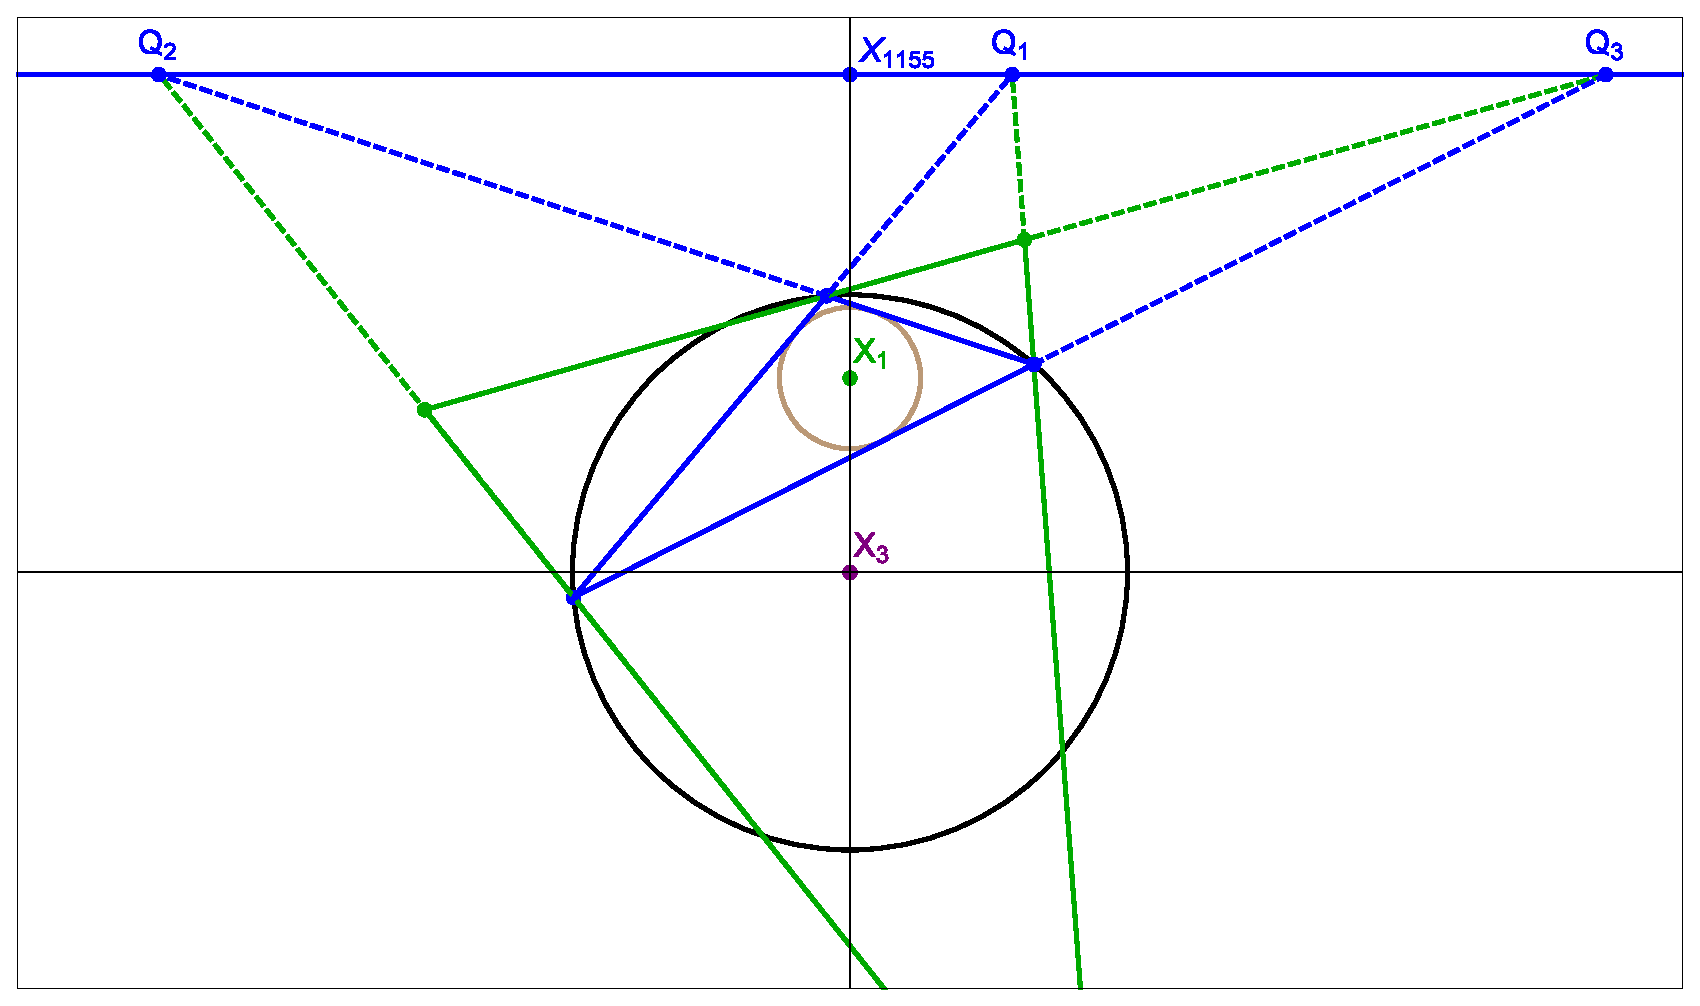
\includegraphics[width=.7\textwidth]{pics_03_220_poristic_antiorthic.eps}
    \caption{Over the poristic family, the antiorthic axis (solid blue) is stationary and perpendicular to $X_1 X_3$. \href{https://youtu.be/DS4ryndDK6Q}{Video}.}
    \label{fig:03-antiorthic}
\end{figure}

In \cite[Antiorthic axis]{mw} the anti-orthic axis is defined as containing the three intersections of a triangle's sidelines with those of the excentral triangle. As illustrated in \cref{fig:03-antiorthic}, the following was proved by \cite{weaver1927-poristic}:

\begin{proposition}
The antiorthic family is stationary over the poristic family and perpendicular to $X_1 X_3$.
\label{prop:03-antiorthic}
\end{proposition}

Let a first vertex $P_1$ of the poristic family be parametrized by $P_1(t)=R[\cos{t},\sin{t}]$.

\begin{proposition}
The perimeter $L(t)$ of poristic triangles is given by:

\begin{equation*}
L(t)=\frac {\left(3\,{R}^{2}
-4\,dR\cos t  +{d}^{2} \right)\sqrt{3\,{R}^{2}+2\,dR\cos t  -{d}^{2}}  }{R\sqrt {{R}^{2}-2\,dR
\cos t  +{d}^{2}}}\\
\end{equation*}
\end{proposition}
\begin{proof}
Follows directly computing the 3-vertices explicitly and using $L(t)=|P_1-P_2|+|P_2-P_3|+|P_3-P_1|$ and simplifying it with a CAS.  
\end{proof}

It turns out poristic triangles can be regarded as the image of billiard 3-periodics (and vice-versa) under (i) a variable similarity transform, and (ii) a polar transformation wrt to a focus-centered circle. We now proceed to prove these results, but first we will need a couple of lemmas.

In \cite[page 17]{odehnal2011-poristic}, one finds the following result, illustrated in \cref{fig:03-poristic-x9}:

\begin{figure}
    \centering
    %\includegraphics[width=.8\textwidth]{pics/0050x_poristic_cb.eps}
    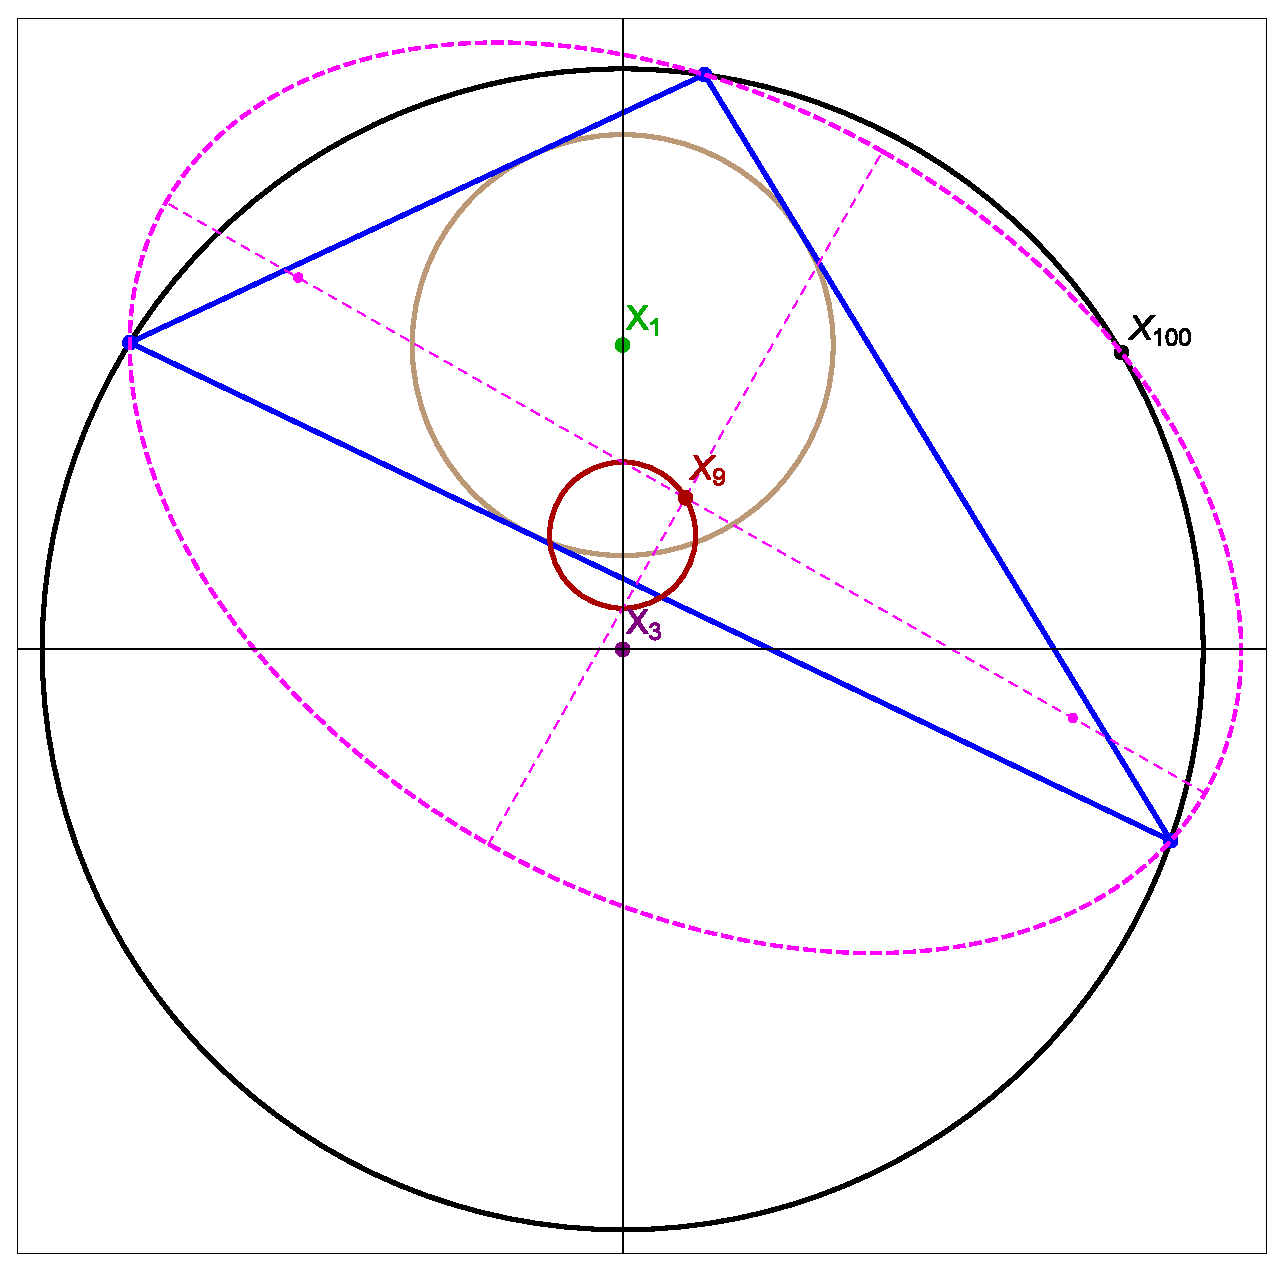
\includegraphics[width=.8\textwidth]{pics_03_190_poristic_cb.eps}
    \caption{A poristic triangles (blue) is shown along as its circumbilliard (dashed magenta) whose aspect ratio is invariant. The locus of the mittenpunkt $X_9$ is a circle (red). \href{https://youtu.be/LGgh11LMGGY}{Video}, \href{https://bit.ly/3tcGtOj}{Live}}
    \label{fig:03-poristic-x9}
\end{figure}

\begin{lemma}
Over the poristic family, the locus of the mittenpunkt $X_9$ is a circle with radius is $R{d^2}R/(9R^2-d^2)$ centered on $X_1 + (X_1 - X_3) (2 R - r)/(4 R + r)=d (3 R^2+d^2)/(9R^2-d^2)$. 
\end{lemma}

In fact we can derive $X_9(t)$ explicitly:

\begin{lemma}
{\small
\begin{align}
    X_9(t)= &\left[  \frac {d \left( 4\, d \mathbf{c}^2   
 \left( R\mathbf{c}_t-d \right) -r \left( 3\,d\mathbf{c}_t  +R \right) -{r}^{2} \right) }{ \left( 4\,R+r \right) 
 \left(d \mathbf{c}_t  -R+r \right) }
  , \, \frac {4R{d}^{2}\mathbf{s}_t  \left( R^2- \left( 2\,R\mathbf{c}_t-d \right) ^{2}  \right) }{ \left( {R}^{2}+{d
}^{2}-2\,dR\mathbf{c}_t  \right)  \left( 9\,{R}^{2}-{d}^{2}
 \right) }
    \right]
\label{eq:03-x9-poristic}
\end{align}
where $\mathbf{c}_t$ and $\mathbf{s}_t$ are shorthand for $\cos(t)$ and $\sin(t)$ respectively.
}
\end{lemma}

Let $P_i=[x_i,y_i]$ denote the vertices of billiard 3-periodics and $P_i'=[x_i',y_i']$ those of a poristic family, $i=1,2,3$.

\begin{theorem}
The $P_i'$ are an image of the $P_i$ under a variable similarity transform comprising of (i) a rigid rotation by $\theta(t)$, (ii) a rigid translation by $X_9(t)$, and (iii)  uniform scaling by $L(t)$. These are given by: 

\begin{align*}
    x_i'=&L(t)(\cos \theta(t) x_i+\sin\theta(t) y_i+x_9(t) )\\
    y_i'=&L(t)(-sin\theta(t) x_i+\cos\theta(t) y_i+y_9(t))\\
    \tan\theta(t)=& \frac{(1-\cos t)(R+d-2R\cos t)}{(2R\cos t+R-d)\sin t}
\end{align*}
\label{thm:similarity}
\end{theorem}

\begin{proof} 
CAS-assisted simplification.
\end{proof}

\cite{reznik2021-circum} term the ``circumbilliard'' $E_9$ of a triangle the circumellipse centered on $X_9$. Let $a_9,b_9$ its semi-axes. CAS manipulation yields:

\begin{corollary}
Over the poristic family, $a_9(t)$ and $b_9(t)$ are given by:
\begin{align*}
a_9=&L(t)\frac{R\sqrt {3\,{R}^{2}+2\,dR-{d}^{2}} }{9\,{R}^{2}-{d}^{2}}\\
b_9=&  L(t)\frac{R\sqrt {R-d}}{\sqrt {3\,R+d} (3\,R-d)}\\
  c_9=&\sqrt{a_9^2-b_9^2}=L(t)\frac{2R\sqrt{dR}}{9R^2-d^2}.
\end{align*}
\end{corollary}

\begin{corollary}
The ratios $a_9(t)/L(t)$, $b_9(t)/L(t)$, and $c_9(t)/L(t)$ are invariant over the Poristic family.
\end{corollary}

\begin{corollary}
Over the poristic family, the aspect ratio of the (varying) circumbilliard is invariant and given by:

\begin{equation*}
\frac{a_9(t)}{b_9(t)}=\sqrt{\frac { \left(  R+d \right)  \left( 3R-d \right) }{ \left( R-d
 \right)  \left( 3\,R+d \right) }}
\end{equation*}
\end{corollary}

In \cite[Polar]{mw}, the {\em polar} of a point $P$ with respect to a circle $\C$ is defined as the line perpendicular to $O P$ which contains the inversion of $P$ wrt to $\C$. Dually, the pole of a line $L$ with respect to $\C$ is the inversion of the foot of the perpendicular dropped from $O$ onto $P$ wrt to $\C$.

So given a smooth curve, we can speak of its {\em polar image} with respect to a circle as the set of poles of the curve's tangents with respect to $\C$. 

\begin{figure}
    \centering
    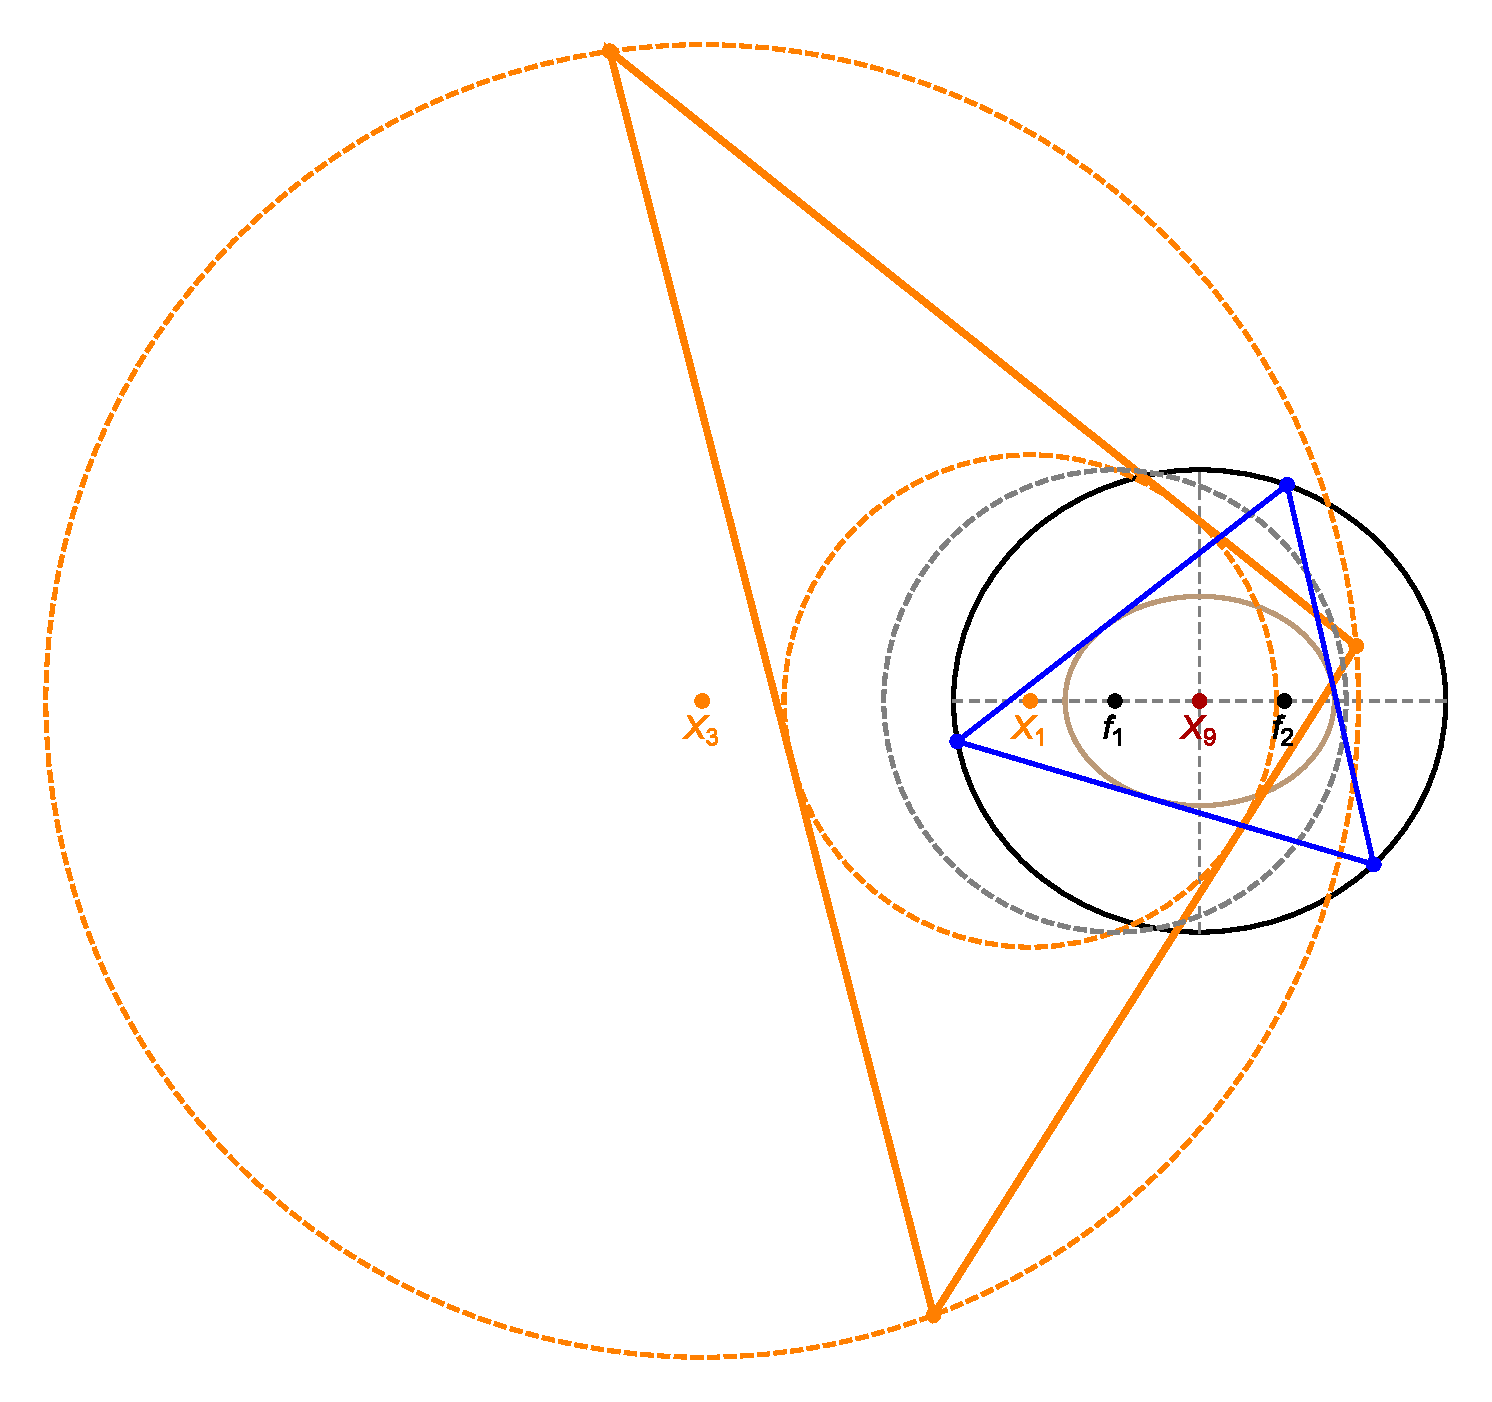
\includegraphics[width=.8\textwidth]{chap_03/pics/pics_03_200_polar_poristic.eps}
    \caption{The poristic family (orange) is the polar image of billard 3-periodics (blue) with respect to a circle (dashed gray) centered on one of the foci of the confocal pair ($f_1$ in the picture). \href{https://bit.ly/3nQ2wcH}{Live}}
    \label{fig:03-polar-poristic}
\end{figure}

The fact that the polar image of an ellipse with respect to a focus is a circle is a well-known result \cite{akopyan2007-conics}.

Let $\E$ and $\E'$ be a confocal ellipse pair centered at $[0,0]$, with major axes along $x$. Let $a,b$ and $a',b'$ denote their major and minor semi-axes, respectively. The foci $f_1$ and $f_2$ are at $[\pm c,0]$, where $c^2=a^2-b^2$. A known classical result which we reproduce below is:

\begin{lemma}
The polar image of the $\E,\E'$ pair with respect to a circle of radius $\rho$ centered on $f_1$ is a pair of nested circles $\C_{int},\C_{ext}$ with centers given by:

\[\O_{int}=[-c-\rho^2\frac{c}{b^2},0],\;\;\;\O_{ext}=[-c-\rho^2\frac{c}{b'^2},0]\]
Their radii $r,R$ and distance $d$ between their centers are given by: 

\[ r=\rho^2\frac{a}{b^2},\;\;\;R=\rho^2\frac{a'}{b'^2},\;\;\; d=\rho^2\frac{ c\, (a^2 - {a'}^2)}{b^2\, {b'}^2} \]
\end{lemma}

%Recall also that a pair of circles uniquely is defines a {\em pencil} of coaxial circles; see \cite[Limiting Points]{mw}. The pencil contains exactly two circles which degenerate to a point, known as {\em limiting points}. A known result is:

%\begin{lemma}
%The limiting points $\ell_1,\ell_2$ of the polar image of a confocal pair $\E,\E'$ with respect to a $f_1$-centered circle are located at $f_1=[-c,0]$ and $[-c+\frac{\rho^2}{c},0]$.
%\end{lemma}
 
Referring to \cref{fig:03-polar-poristic}:

\begin{corollary}
The poristic family is the polar image of billiard 3-periodics with respect to a circle centered on a focus. 
\end{corollary}

\begin{corollary}
The sum of cosines of the polar image of billiard 3-periodics with respect to a focus-centered circle is given by:

\begin{equation}
\sum\cos\theta' = 1+\frac{r}{R} = 1+\frac{a b'^2}{a' b^2}
\label{eq:03-bic-cos}
\end{equation}
\end{corollary}

\begin{figure}
    \centering
    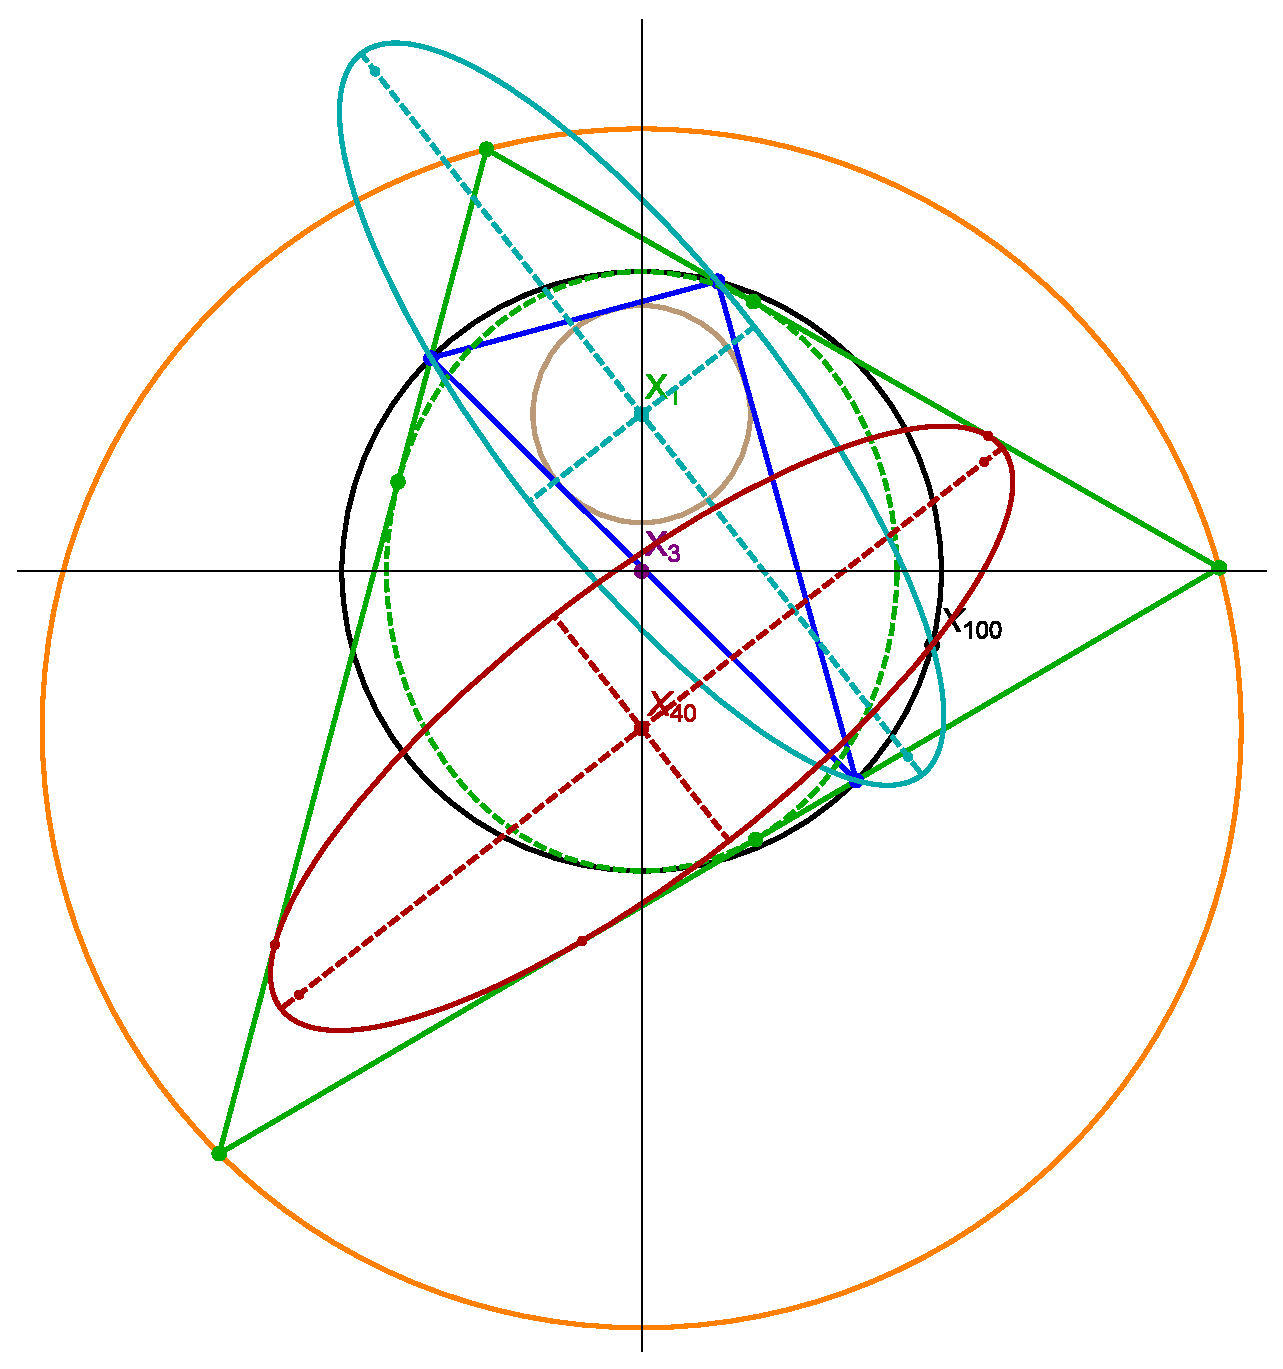
\includegraphics[width=.7\textwidth]{pics_03_230_excentral_poristic_inconics.eps}
    \caption{A poristic triangle (blue) is shown, as well as $I_1$, the $X_1$-centered inconic (light blue). Also shown is the excentral triangle (green), the circle (orange) the excentral family is inscribed in and their MacBeath caustic (dashed green). Also shown is $I_3'$ (dark red), the $X_3'$-centered excentral inconic (red). Note $X_3'=X_{40}$. Over the poristic family, both $I_1$ and $I_3'$ rotated rigidly at 90-degrees from each other. \href{https://youtu.be/hz0qEyVVvaI}{Video}}
    \label{fig:03-excentral-poristic-inconics}
\end{figure}

Given a triangle, an inconic is is fully defined by its center and is tangent to the three sidelines, see \cite[Inconic]{mw}.

Referring to \cref{fig:03-excentral-poristic-inconics}, let $E_1$ be the $X_1$-centered inconic to the poristic family. Let $\mu_1$, and $\nu_1$ denote its semi-axes. Interestingly:

\begin{proposition}
$\mu_1=R+d$ and $\nu_1=R-d$ are invariant over the poristic family, i.e., $E_1$ rigidly rotates about $X_1$. \label{prop:03-e1}
\end{proposition}

A proof appears in \cite[Appendix C]{garcia2020-similarity-I}.

\subsection{Poristic Excentrals}

\begin{figure}
    \centering
    %\includegraphics[width=.7\textwidth]{pics/0170_poristic.eps}
    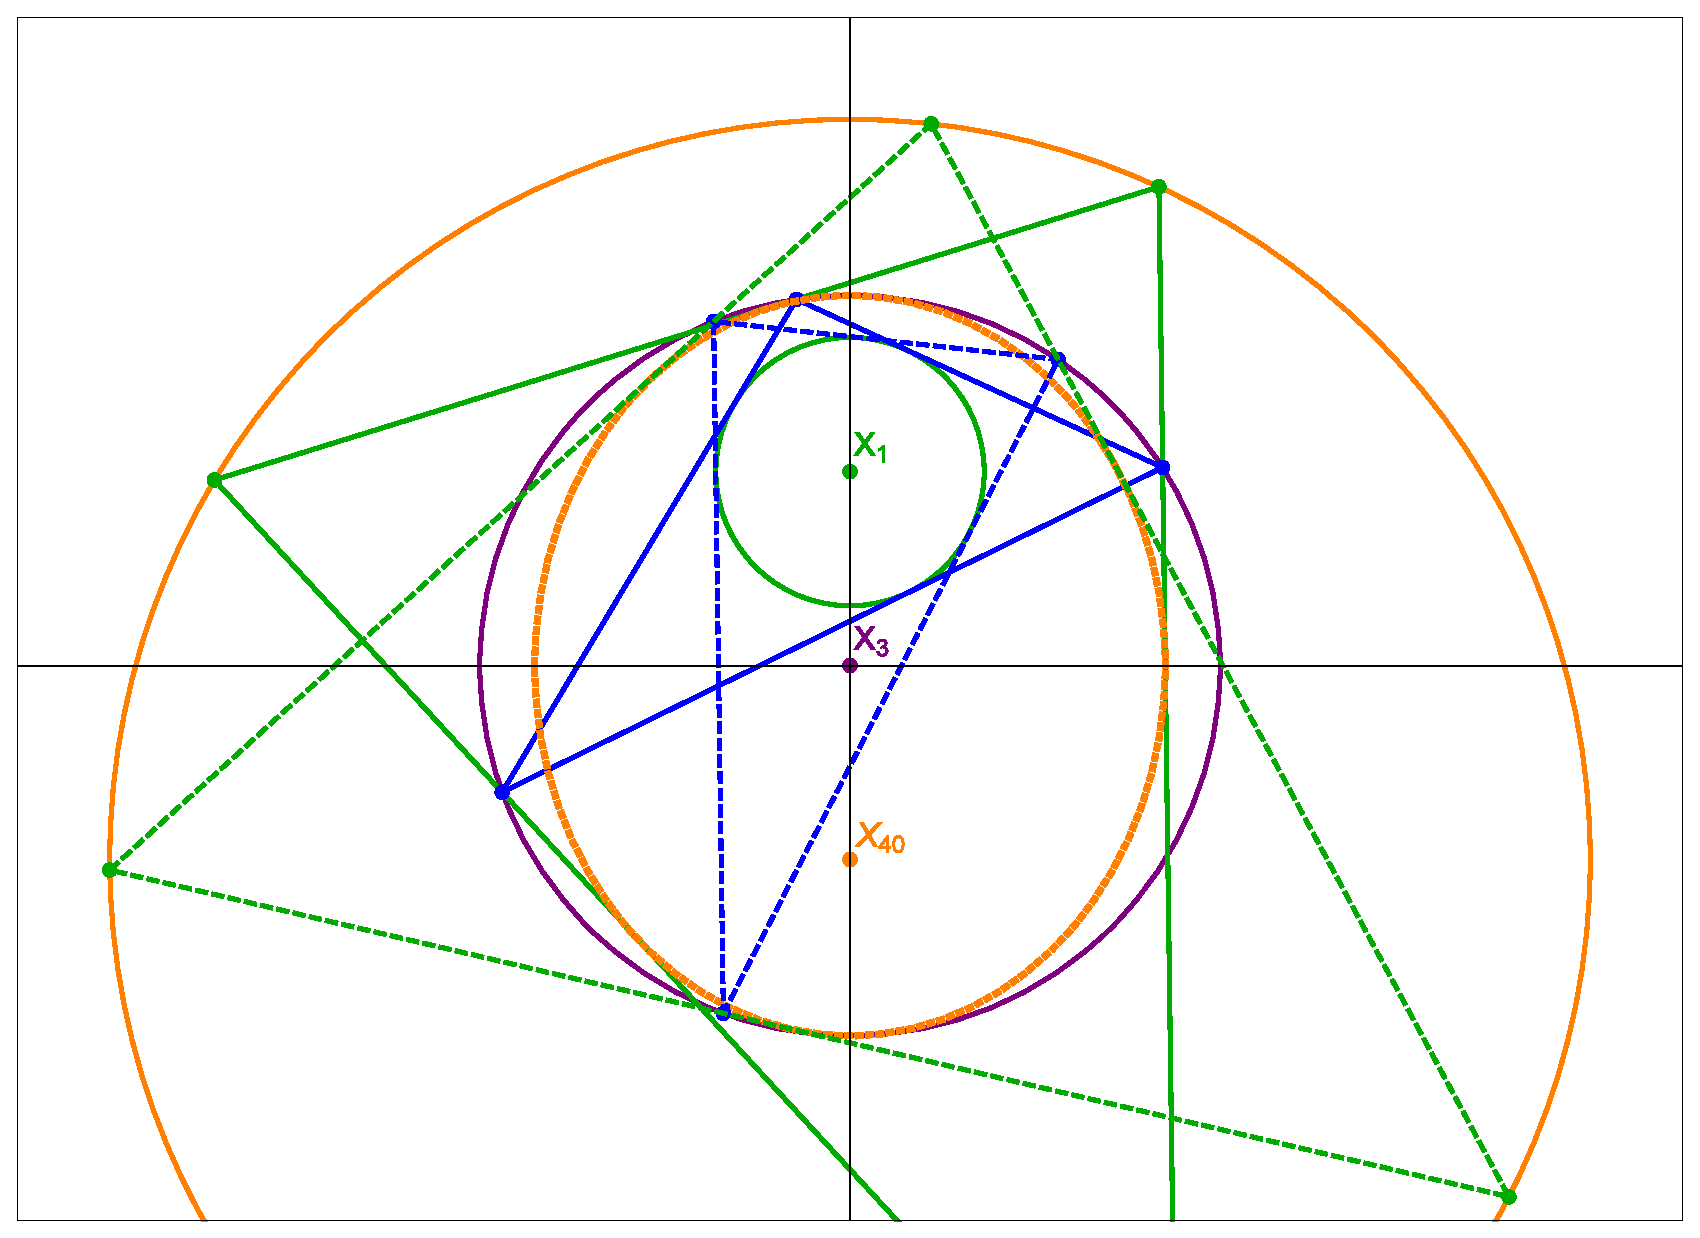
\includegraphics[width=\textwidth]{pics_03_170_poristic.eps}
    \caption{The poristic family (blue) is interscribed between two fixed circles, i.e., their circumcenter $X_3$ and incenter $X_1$ are stationary. The family of its excentral triangles (solid green) are inscribed in a circle (orange) centered on the Bevan point $X_{40}$ and of radius twice the original circumradius. This family circumscribes the MacBeath inellipse (dashed orange), centered on $X_3$ with foci on $X_1$ and $X_{40}$. A second for both poristics and excentrals configuration is also shown (dashed blue and dashed green).  \href{https://youtu.be/DS4ryndDK6Q}{Video}, \href{https://bit.ly/2RoYJHm}{Live}}
    \label{fig:03-poristic-excentrals}
\end{figure}

The family of excentral triangles to the poristic family, shown in \cref{fig:03-poristic-excentrals} is also Ponceletian: in \cite{odehnal2011-poristic}, it is shown to be inscribed in a circle of radius $2R$ where $R$ is the circumradius of its reference poristic family, centered on $X_{40}$, the Bevan point, or $X_3'$ of the family in questions (to avoid confusion, we will be priming quantities associated with this family).

\begin{proposition}
The barycenter $X_2'$ of poristic excentrals is stationary.
\end{proposition}

\begin{proof}
Recall a triangle's barycenter $X_2$ is a third of the way from the circumcenter to the orthocenter \cite[Euler Line, Eqn. 6]{mw}. The result follows from the fact that both $X_3'=X_{40}$ and $X_4'=X_1$ are stationary.
\end{proof}

The MacBeath inconic, defined in \cite[MacBeath Inconic]{mw}, is an ellipse centered on a triangle's 9-point center $X_5$, with  foci at the circumcenter $X_3$ and orthocenter $X_5$.

Poristic excentrals are Ponceletian since:

\begin{proposition}
The MacBeath inconic to the excentral poristics is stationary and is therefore the caustic. Let $\mu_5'$ and $\nu_5'$ denote its major and minor semi-axes. These are given by:
\[ \mu_5'=R,\;\;\;\nu_5'=\sqrt{R^2-d^2} \]
\end{proposition}

\begin{proof}
It is straightforward to verify the sidelines of poristic excentrals are dynamically  tangent to the ellipse:
\[
\frac{(x-d)^2}{R^2}+\frac{y^2}{R^2-d^2}=1\]
with center $X_3=(d,0)$ and foci $X_{40}=(0,0)$ and $X_1=(2d,0)$.
\end{proof}

Correspondences between the centers and foci of the excentral MacBeath inconic and those of the reference triangle appear in \cref{tab:03-macbeath}.

\begin{table}
\centering
\begin{tabular}{|c|c|c|}
\hline
\makecell[cc]{excentral\\ MacBeath} &
\makecell[cc]{excentral\\center} &
\makecell[cc]{reference\\center} \\
\hline
center & $X_5'$ & $X_3$\\
focus & $X_4'$ & $X_1$  \\
focus & $X_3'$ & $X_{40}$ \\
\hline
\end{tabular}
\caption{Center and foci of the MacBeath inconic of an excentral triangle and the corresponding triangle center of the reference.} 
\label{tab:03-macbeath}
\end{table}

Since $\mu'_5/\nu_5'=R/\sqrt{R^2-d^2}$, use \cref{eq:03-euler-poristic} to obtain:

\begin{corollary}
The aspect ratio of the caustic to the excentral poristics is given by:
\begin{equation*}
 \frac{\mu'_5}{\nu_5'}={\sqrt\frac{R}{2 r}}
\end{equation*}
\end{corollary}

As shown in \cref{fig:03-excentral-poristic-inconics}, let $I_3'$ be the $X_3'$-centered inconic to poristic excentrals. Let $\mu_3'$ and $\nu_3'$ denot its major and minor semi-axes, respectively.

\begin{proposition}
Over poristic excentrals,  $\mu_3'=R+d$ and $\nu_3'=R-d$ are invariant, i.e., $I_3'$ rigidly rotates about $X_3'$.
\label{prop:03-inconic-x3p}
\end{proposition}

We omit the long proof kindly contributed by B. Odehnal and appearing in \cite[Appendix C]{garcia2020-similarity-I}.

Interestingly:

\begin{theorem}
Excentral poristics are the image of the circumcircle family under a variable rigid rotation. The ridigly-rotating $I_3'$ is identified with the caustic of the circumcircle family.
\end{theorem} 

\begin{proof}
Recall \cref{prop:03-circumcircle-rh}: the orthic triangles of the circumcircle family has invariant inradius and circumradius. Also recall \cref{lem:03-circum-x5-locus}: the locus of the orthic circumcenter is a circle concentric with the common center. Also notice in the circumcircle family, the caustic is the stationary inconic centered on $X_3$.
\end{proof}

\subsection{The Brocard Porism}
 
A property-rich family of Poncelet triangles is the so-called ``Brocard porism'', introduced in  \cite{bradley2007-brocard,shail1996-brocard, bradley2011-brocard}. It is inscribed in a circle and circumscribes the so-called {\em Brocard inellipse}. Remarkably, its foci coincide with the stationary Brocard points $\Omega_1$ and $\Omega_2$ of the family; see \cref{fig:03-brocard-porism}.

Let $R$ denote the radius of the outer circle and $a,b$ the caustic semi-axes, with $c=a^2-b^2$. \textcolor{red}{should be $a',b'$?}

\begin{proposition}
The stationary circumcenter $X_3$ and circumradius $R$ are given by:

\begin{equation}
X_3=[0,-\frac{c\delta_1}{b}],\;\;\;R= \frac{2a^2}{b} \\
 %=& \frac{\sqrt{3a^2+2c^2-2c\delta_1} (c +\delta_1)\delta_1}{ 3a^2b} 
 \label{eqn:broc-circumcircle}
\end{equation}
where $\delta_1=\sqrt{4a^2-b^2}$.
\label{prop:cotw}
\end{proposition}

The following is a known requirement for the Brocard porism to be possible, appearing in \cite[Eqs. 15--17]{shail1996-brocard}:

\begin{corollary}
$R{\geq}2c$
\label{rem:minR}
\end{corollary}

Remarkably, and echoing a property seen above for the homothetic family, leaving the proof as an exercise:

\begin{proposition}
Over the Brocard porism, the Brocard angle $\omega$ is invariant and given by:
\[\cot\omega=\frac{\delta_1}{b} \geq \sqrt{3} \]
\label{prop:03-brocard-w}
\end{proposition}

Recall for any triangle $\cot\omega=\sum_{i=1}^3{\cot{\theta_i}}$, i.e.:

\begin{corollary}
The Brocard porism conserves the sum of its internal angle cotangents.
\end{corollary}

\cite{shail1996-brocard} derives the distance between Brocard points in terms of invariant $R$ and $\omega$:

\[ |{\Omega_1}-{\Omega_2}|^2=4 R^2\sin^2{\omega}(1-4\sin^2{\omega})
\]

Since the $\Omega_i$ are foci of the caustic, and therefore $|{\Omega_1}-{\Omega_2}|^2= c^2$, obtain:

\begin{corollary}
\[ c = R\sin{\omega}\sqrt{1-4\sin^2{\omega}} \]
\end{corollary}
 
 \begin{figure}
     \centering
     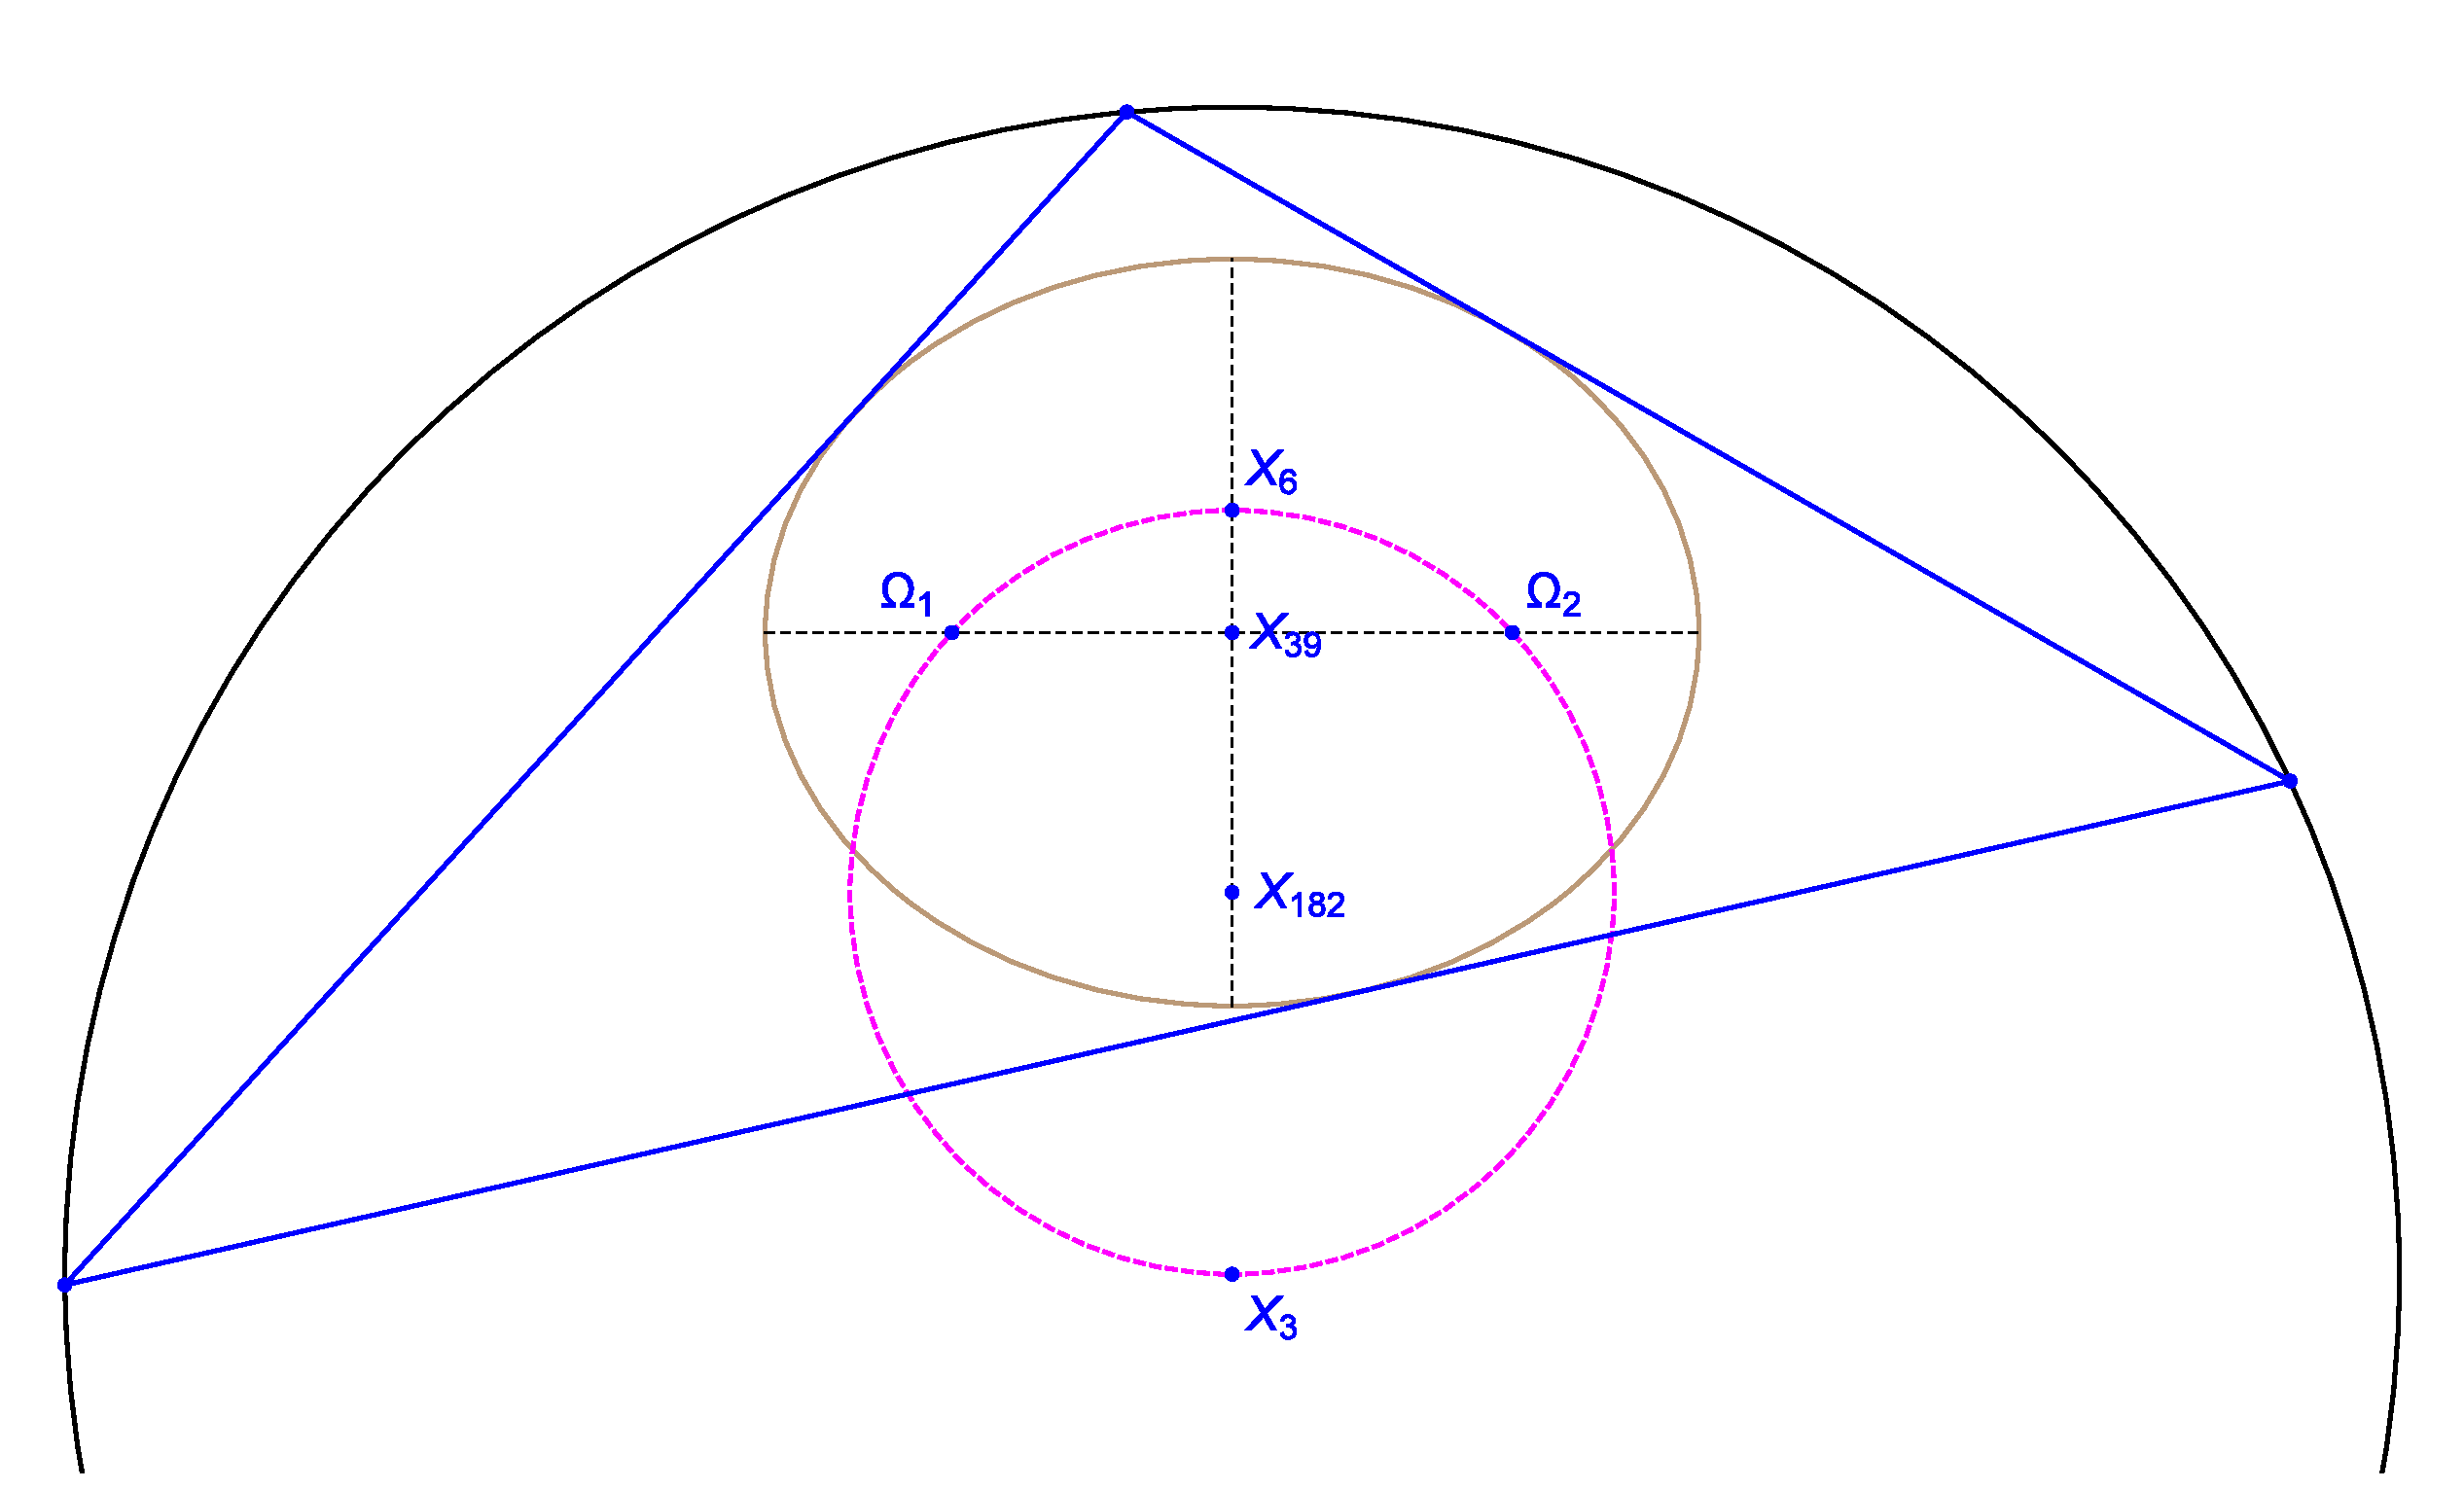
\includegraphics[width=\textwidth]{pics_03_240_brocard_porism.eps}
     \caption{A triangle (blue) in the Brocard porism is shown inscribed in an outer circle (black) and having the Brocard inellipse (brown) as its caustic, with foci at the stationary Brocard points $\Omega_1$ and $\Omega_2$ of the family, and centered on the Brocard midpoint $X_{39}$. The Brocard points as well as the stationary circumcenter $X_3$ and symmedian point $X_6$ are concyclic on the Brocard circle (dashed magenta), whose center is $X_{182}$. \href{https://bit.ly/2QX3lEt}{Live}}
     \label{fig:03-brocard-porism}
 \end{figure}

Referring to \cref{fig:03-brocard-porism}, all of $\Omega_1$, $\Omega_2$, $X_3$, and $X_6$ are concyclic on the so-called Brocard circle, see \cite[Brocard Circle]{mw}, whose center is $X_{182}$. The Brocard axis is defined in \cite[Brocard Axis]{mw} as the line containing the circumcenter $X_3$ and symmedian point $X_6$ of a triangle.
 
\begin{proposition}
Over the Brocard porism, the following 3 objects are stationary: (i) the Brocard circle, (ii) the Brocard axis, and (iii) the symmedian point $X_6$ are stationary.
\end{proposition}

\begin{proof}
The Brocard circle is stationary since it passes through 3 stationary points: $\Omega_1,\Omega_2,X_3$ are stationary. The Brocard axis is stationary since it contains stationary $X_3$ and stationary Brocard midpoint $X_{39}$. For any triangle, $X_6$ is antipodal to $X_3$ on the Brocard circle.
\end{proof}
 
Recall the two isodynamic points $X_{15}$ and $X_{16}$ of a triangle as the two unique intersections of the 3 Apollonius circles\footnote{These are circles which contain a vertex and the intersection of the corresponding internal and external bisectors with the opposite side.}. $X_{15}$ (resp. $X_{16}$) is interior (resp. exterior) to the circumcircle. In fact they are inverse images of each other with respect to the latter, see \cite[Isodynamic Points]{mw}.

\begin{proposition}
Over the Brocard porism, the two Isodynamic points $X_{15}$ and $X_{16}$ are stationary and given by:

\[
X_{15}=\left[0, \frac{R(\sqrt{3}-\cot{\omega})}{
 \sqrt{\cot^2{\omega}-3}}\right],\;\;\;
 X_{16}=\left[0, -\frac{R(\sqrt{3}+\cot{\omega})}{
 \sqrt{\cot^2{\omega}-3}}\right]
\]
\label{prop:03-x15x16}
\end{proposition}

\begin{proof}
Let $P$ and $U$ be finite points on a triangle's plane with normalized barycentric coordinates $(p,q,r)$ and $(u,v,w)$, respectively. Let $f$ and $g$ be homogeneous functions of the sidelengths. The $(f,g)$ {\em barycentric combo} of $P$ and $U$, also denoted $f*P + g*U$, is the point with barycentrics $(f\,p + g\,u,f\,q + g\,v, f\,r + g\,w)$. In \cite[X(15), X(16)]{etc}, the following combos (see below), derived by Peter Moses, are provided:

\begin{align}
X_{15} =& \sqrt{3}*X_3 + \cot{\omega}*X_6 \label{eqn:combo-x15} \\
X_{16} =& \sqrt{3}*X_3 - \cot{\omega}*X_6 \nonumber
\end{align}
 
 With all involved quantities invariant, the result follows.
\end{proof}

\begin{proposition}
The semi-axes $(a,b)$ and center $X_{39}$ of the Brocard inellipse are given by:

\begin{gather*}
[a,b]= R\left[\sin\omega,2\sin^2\omega\right]=R\left[\frac{1}{\sqrt{1+\Sha^2}},\frac{2}{{1+\Sha^2}}\right]\\
 X_{39}=\left[0,-\frac{R\Sha\sqrt{\Sha^2-3}}{\Sha^2+1}\right]
\end{gather*}
 \label{prop:03-brocard-axes}
\end{proposition}

\begin{proof}

Consider a triangle $T$ with sidelengths $s_1,s_2,s_3$, area  $\Delta$, and circumradius  $R$. The following identities appear in \cite{bradley2007-brocard,shail1996-brocard}:

\[R=\frac{s_1 s_2 s_3}{4\Delta}, \;\;\; \sin\omega=\frac{2\Delta}{\sqrt{\Gamma}},\;\;\; |\Omega_1-\Omega_2|^2=4c^2=4R^2\sin^2\omega (1-4\sin^2\omega)\]

\noindent where $\Gamma=(s_1 s_2)^2+(s_2 s_3)^2+ (s_3 s_1)^2$, and $c^2=a^2-b^2$. The result follows from combining the above into expressions for the Brocard inellipse semi-axes given in \cite[Brocard Inellipse]{mw}:

\[ a =\frac{s_1 s_2 s_3}{2\sqrt{\Gamma}},\;\;\;\;\;\; b =\frac{2 s_1 s_2 s_3 \Delta}{\Gamma}.\]

\end{proof}

With the results above, we can derive the following quantities and centers explicitly:

\begin{align*}
X_6&=\left[0,-\frac{R\sqrt{ \Sha^2 -3}}{ \Sha}\right] \\
|X_3-X_6|&=\frac{R\sqrt{ \Sha^2 -3}}{ \Sha}\\
\Omega_{1,2}(R,\Sha)&=\frac{R\sqrt{ \Sha^2-3}}{ \Sha^2+1} \left[\pm1, - \Sha  \right]\\
X_{39}&=\left[0,-R {\frac {\Sha\,
\sqrt {\Sha^2-3}}{\Sha^2+1}} \right]
\end{align*}

Introduced here for the first time is the following conservation unique to the Brocard porism:
 
 \begin{proposition}
 Over the Brocard porism, the sum of inverse squared sidelengths is invariant and given by:
 
\textcolor{red}{ronaldo consegue expressar em termos de $R$, ou $a,b$ da caustica? esta notacao $d,h$ acho pode ser antiga}
\[ \sum{s_i^{-2}}=\frac{9 d^2 + h^2}{ 4 d^2 \,(d^2 + h^2)}\]
\label{prop:03-sum-inverse-brocard}
\end{proposition}

\begin{itemize}
    \item Brocard porism is a variable image of the homothetic family under a variable similarity transform.
    \item Brocard porism is the polar image of the homothetic family wrt to a focus-centered circle.
\end{itemize}

\subsection{General Case}

\begin{table}
\centering
\begin{tabular}{|r|c|c|l|}
\hline
Family & Fixed & Conserves & Notes \\
\hline
\makecell[rc]{Poristic\\(bicentric)} & $X_1$, $X_3$, $X_{40}$, $\ldots$ & $\sum\cos\theta_i,a_9/b_9$ & \makecell[lc]{polar image of Confocal family\\wrt to a focus} \\
\hline
\makecell[rt]{Poristic\\Excentrals} & $X_2$, $X_3$, $X_4$, $X_5$ & $\sum{s_i^2}$, $\prod\cos\theta_i$ & \makecell[lt]{Inscribed in circle;\\caustic is MacBeath inconic} \\
\hline
Brocard & \makecell[lc]{$X_3$, $X_6$, $X_{15}$, $X_{16}$,\\$X_{39}$, $X_{182},\ldots$,\\$\Omega_1$, $\Omega_2$} & $\sum{s_i^{-2}}$, $\omega$, $\sum\cot\theta_i$ & \makecell[lc]{polar image of Homothetic\\family wrt caustic focus;\\inscribed in circle;\\caustic is Brocard inellipse}\\
%\hline
%focus-Inversive & $X_7$ & $L,\sum\cos\theta_i$ & \makecell[lc]{inversive image of Confocals\\wrt a focus; non-Ponceletian;\\inscribed in Pascal's limaçon;\\caustic non-ellipse}\\
\hline
\end{tabular}
\caption{Some Non-concentric, axis parallel families, their stationary triangle centers, and known conservations.}
\label{tab:n3-non-conc-families}
\end{table}
